L'évolution rapide des technologies numériques a radicalement transformé les attentes des consommateurs. Dans un marché e-commerce de plus en plus concurrentiel, la qualité du service client est devenue un différenciateur aussi critique que la qualité des produits eux-mêmes. Ce projet s'inscrit dans cette dynamique de transformation en proposant une solution d'\gls{agentia} de nouvelle génération.

\section{Contexte du projet}

L'origine de ce projet réside dans un constat opérationnel critique observé sur les plateformes de commerce en ligne ciblant le marché africain (zones francophones et arabophones). Les services de support client traditionnels font face à une triple contrainte :

\begin{enumerate}
    \item \textbf{Saturation des canaux :} L'augmentation exponentielle des interactions clients sature les équipes humaines, entraînant des délais de réponse inacceptables.
    \item \textbf{Complexité linguistique :} La nécessité de traiter simultanément le Français et l'Arabe (littéraire et dialectal) crée une barrière à l'entrée pour les solutions d'automatisation standards.
    \item \textbf{Limites des Chatbots actuels :} La majorité des solutions déployées reposent sur des arbres de décision rigides ou du \gls{nlp} basique. Elles échouent dès que la requête nécessite un raisonnement contextuel ou une interaction avec le système d'information (\gls{erp}).
\end{enumerate}

Dans ce contexte, l'émergence des \gls{llm} et des techniques de \gls{rag} offre une opportunité technologique majeure. Cependant, l'approche classique basée uniquement sur une \gls{vectordatabase} montre ses limites pour des questions techniques nécessitant une compréhension fine des relations entre produits (compatibilité, hiérarchie).

C'est pour pallier ces insuffisances que nous nous sommes tournés vers l'\gls{ingenierieconnaissances} et le \gls{websemantique}, en proposant une transition vers une architecture \gls{knowledgegraph}.

% --- DIAGRAMME DE CONTEXTE ---
\begin{figure}[h]
    \centering
    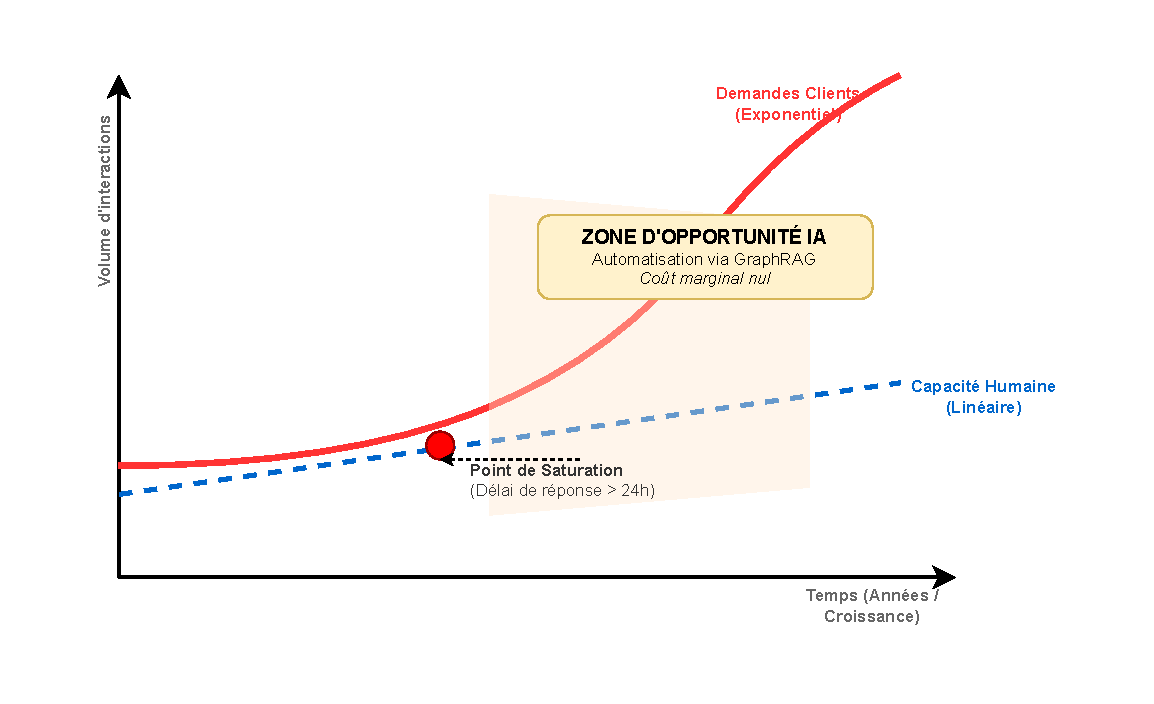
\includegraphics[width=1\textwidth]{docs/contexte_market.pdf}
    
    \caption{\textbf{Modélisation du "Ciseau Opérationnel" (Scalability Gap).} 
    Illustration théorique de la divergence entre la croissance exponentielle du trafic e-commerce et la capacité linéaire de recrutement des agents humains. 
    \textit{(Source : Projection basée sur les tendances standards de l'industrie Customer Care).}}
    \label{fig:contexte}
\end{figure}

\section{Objectifs}

L'ambition de ce projet est de concevoir, développer et déployer un prototype fonctionnel d'un assistant intelligent autonome. Pour garantir le succès de cette initiative, nous avons défini des objectifs selon la méthode SMART :

\begin{itemize}
    \item \textbf{Spécifique (S) :}
    Développer une \gls{architecturehybride} combinant trois moteurs décisionnels : un moteur transactionnel pour le suivi de commande, un moteur \gls{graphrag} basé sur \gls{neo4j} pour le raisonnement complexe, et un moteur sémantique classique. L'agent doit être capable d'interagir en temps réel via \gls{websocket}.

    \item \textbf{Mesurable (M) :}
    \begin{itemize}
        \item Atteindre un taux d'automatisation supérieur à \textbf{80\%} sur les questions de niveau 1 et 2.
        \item Maintenir un temps de latence (\gls{inference}) inférieur à \textbf{2.5 secondes}.
        \item Obtenir un taux de précision supérieur à \textbf{90\%} sur les questions relationnelles (ex: "Qui fabrique ce produit ?") grâce à l'\gls{ontologie} définie.
    \end{itemize}

    \item \textbf{Atteignable (A) :}
    Le projet s'appuie sur des technologies éprouvées et modernes : \gls{langchain} pour l'orchestration, \gls{conteneurisation} via Docker pour la portabilité, et l'API Google Gemini pour la génération. L'intégration des données se fera via des pipelines d'\gls{embedding} et de \gls{chunking} optimisés.

    \item \textbf{Réaliste (R) :}
    Le périmètre est circonscrit à un agent de support client e-commerce. La connexion à l'\gls{erp} est simulée via un Mock Service pour se concentrer sur la logique de l'\gls{orchestrateur} et la qualité du \gls{nlu}.

    \item \textbf{Temporel (T) :}
    Le développement est structuré en 6 Sprints intensifs, allant de la mise en place de l'infrastructure à l'intégration de la mémoire via \gls{redis} et au peaufinage du \gls{promptengineering}.
\end{itemize}

\section{Problématique}

Au cœur de ce projet se trouve une tension fondamentale entre la flexibilité des modèles de langage et la rigueur nécessaire aux processus métiers.

Si les \gls{llm} excellent dans la génération de texte fluide, ils souffrent d'un défaut majeur en entreprise : l'\gls{hallucination}. D'un autre côté, les bases de données relationnelles ou les graphes sémantiques (\gls{cypher}) offrent une vérité absolue mais sont difficiles à interroger en langage naturel pour un utilisateur lambda.

La problématique centrale à laquelle ce projet tente de répondre est donc la suivante :

\begin{quote}
\textbf{\textit{Comment concilier la puissance générative des LLM avec la rigueur structurelle des Graphes de Connaissances pour créer un agent conversationnel capable de raisonner de manière fiable et empathique dans un contexte multilingue ?}}
\end{quote}

Cette question soulève plusieurs défis sous-jacents que nous aborderons :
\begin{enumerate}
    \item Comment structurer les données non structurées (PDF, FAQ) en un \gls{knowledgegraph} exploitable ?
    \item Comment orchestrer dynamiquement les appels entre une \gls{api} externe, une base vectorielle et une base de graphe ?
    \item Comment doter l'agent d'une mémoire contextuelle tout en gérant les contraintes de tokens et de coûts ?
\end{enumerate}

% --- DIAGRAMME DU FOSSÉ COGNITIF ---
\begin{figure}[h]
    \centering
    % Sauvegardez le diagramme Draw.io sous le nom 'problematique_gap.png'
    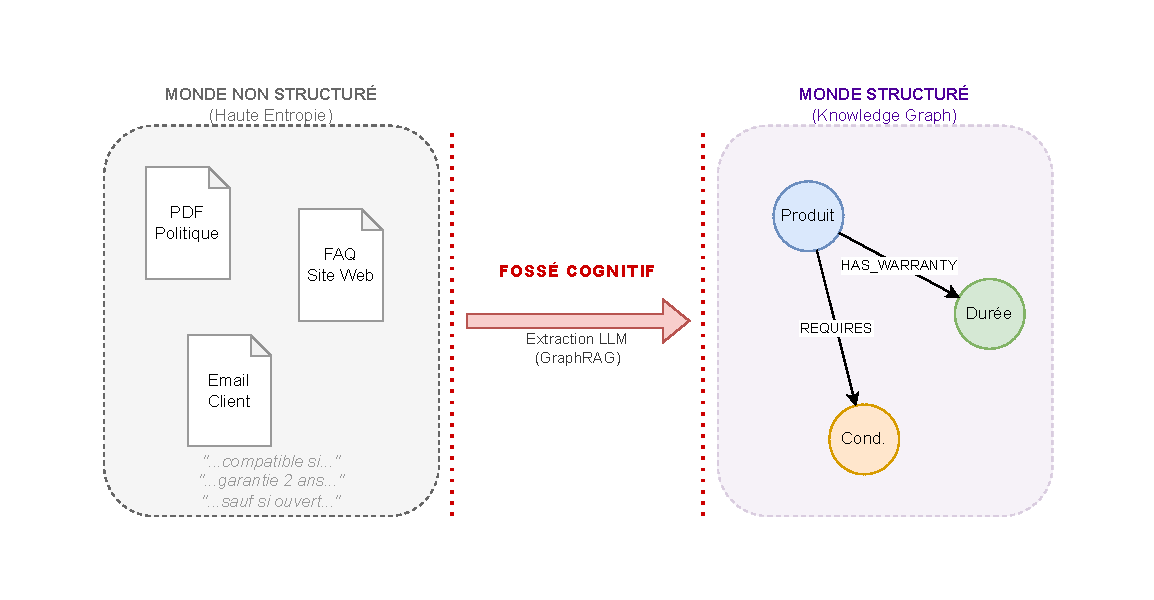
\includegraphics[width=0.9\textwidth]{docs/problematique_gap.pdf}
    
    \caption{\textbf{Le Fossé Cognitif (The Cognitive Gap).} 
    Représentation du défi central du projet : comment passer d'une masse d'informations non structurées (documents, texte libre) à une structure de connaissance exploitable par une machine (Graphe), sans intervention humaine manuelle. C'est ce fossé que le GraphRAG permet de franchir.}
    \label{fig:problematique}
\end{figure}